%% question-7.tex
%%

%% ==============================
\subsection{Modélisation du concept de stratégie}
\label{sec:question7}
%% ==============================

Voici un diagramme de classe qui fixe les éléments principaux d'une stratégie :

Une \emph{Stratégie} est composé d'une \emph{vision court terme} et une \emph{vision long terme} qui sont toutes les deux articulées par des \emph{Objectif} eux même réalisés par des \emph{Règle}.

Une \emph{Stratégie} comporte également des \emph{Déclaration} pouvant être des \emph{Module} ou des \emph{Variable}.

\begin{figure}
	\centering
	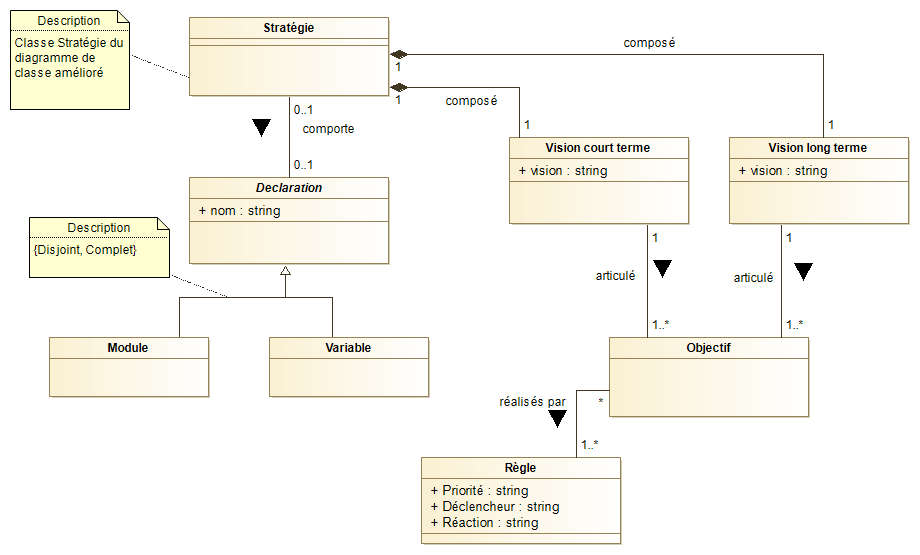
\includegraphics[width=500pt]{assets/strat_base}
	\caption{Diagramme de classe d'une stratégie}
	\label{fig:strategie}
\end{figure}